\newcommand{\screenShotSize}{400pt}
\hyphenation{'certificats'}


\section{Windows}


\subsection{Connection en challenge-MD5}

Allez dans le panneau des connections.\\
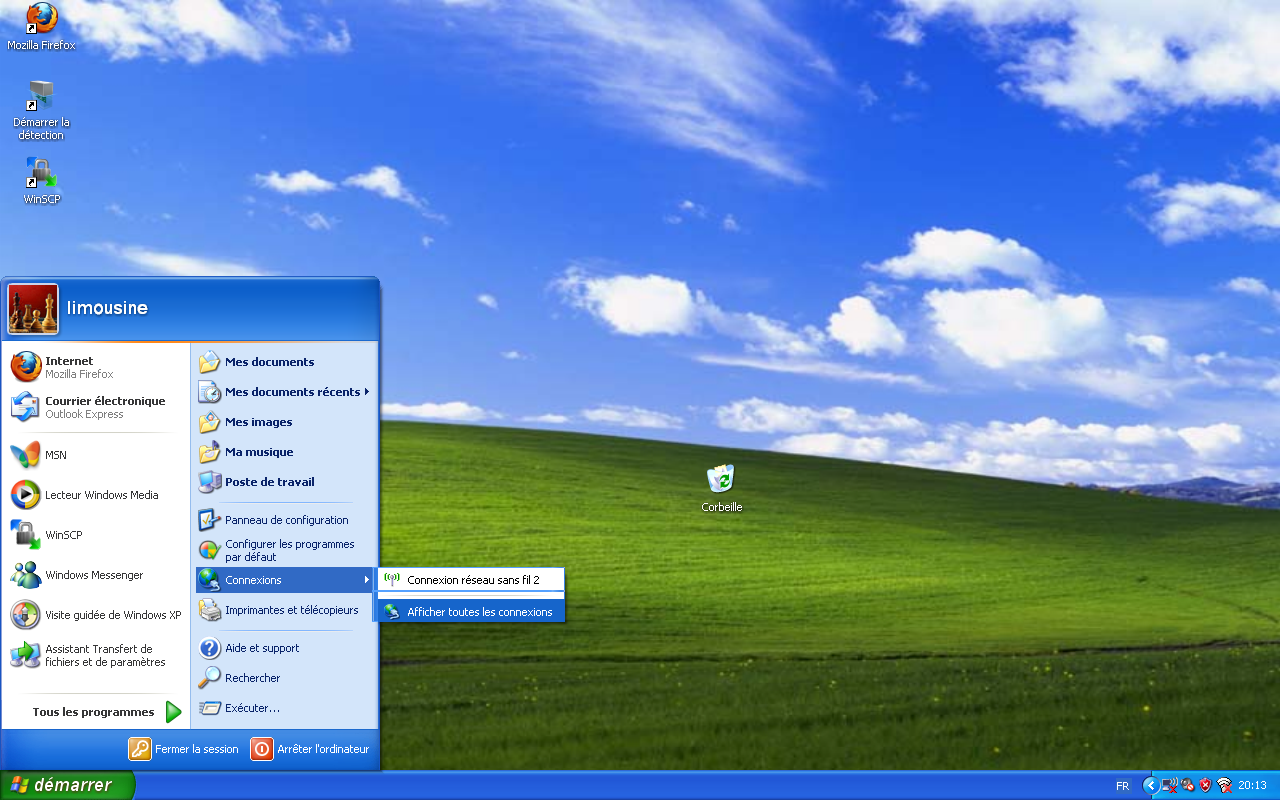
\includegraphics[width=\screenShotSize{}]{imgUser/connections.PNG}\\
Puis effectuez un clic droit sur la connexion que vous utilisez pour accéder au reseaux, et ouvrez les propriétés de la connexion.\\
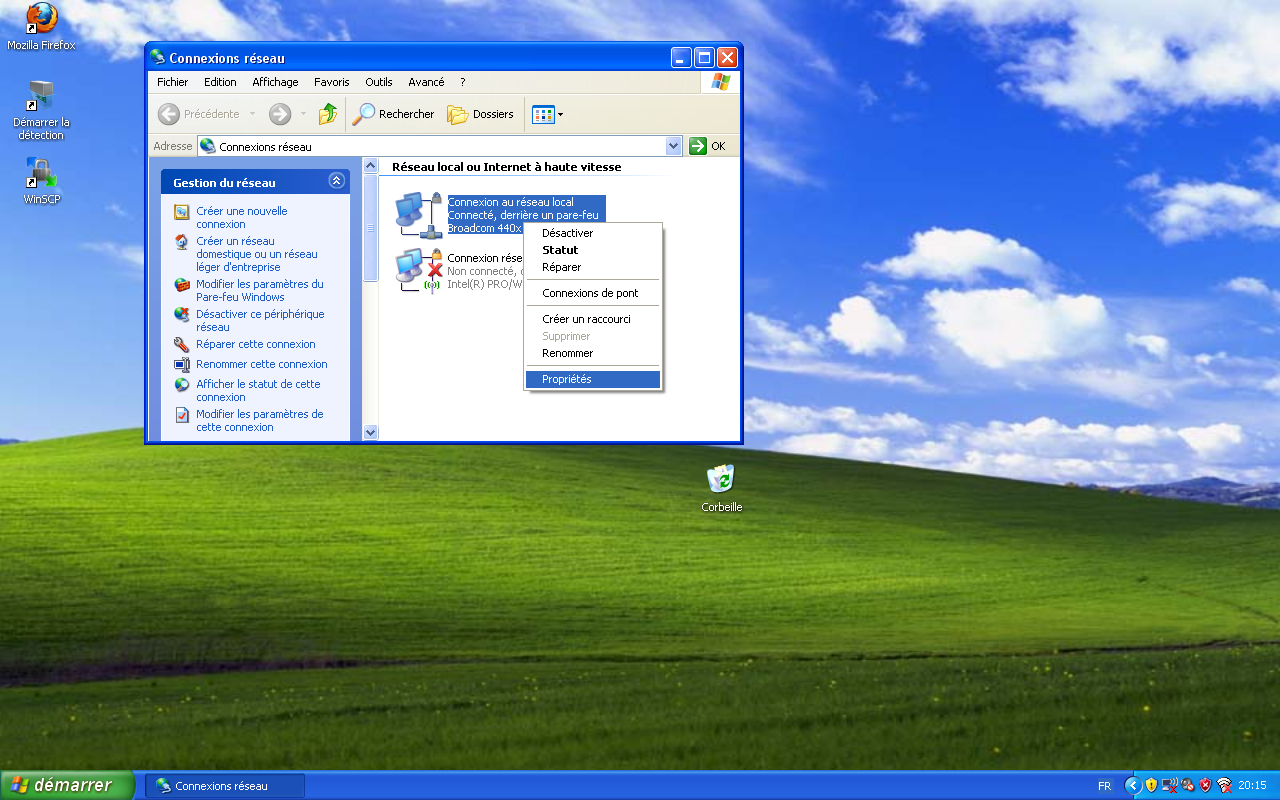
\includegraphics[width=\screenShotSize{}]{imgUser/connectionProperties.PNG}\\
Choisissez alors 'challenge-MD5' dans l'onglet 'Authentification'.\\
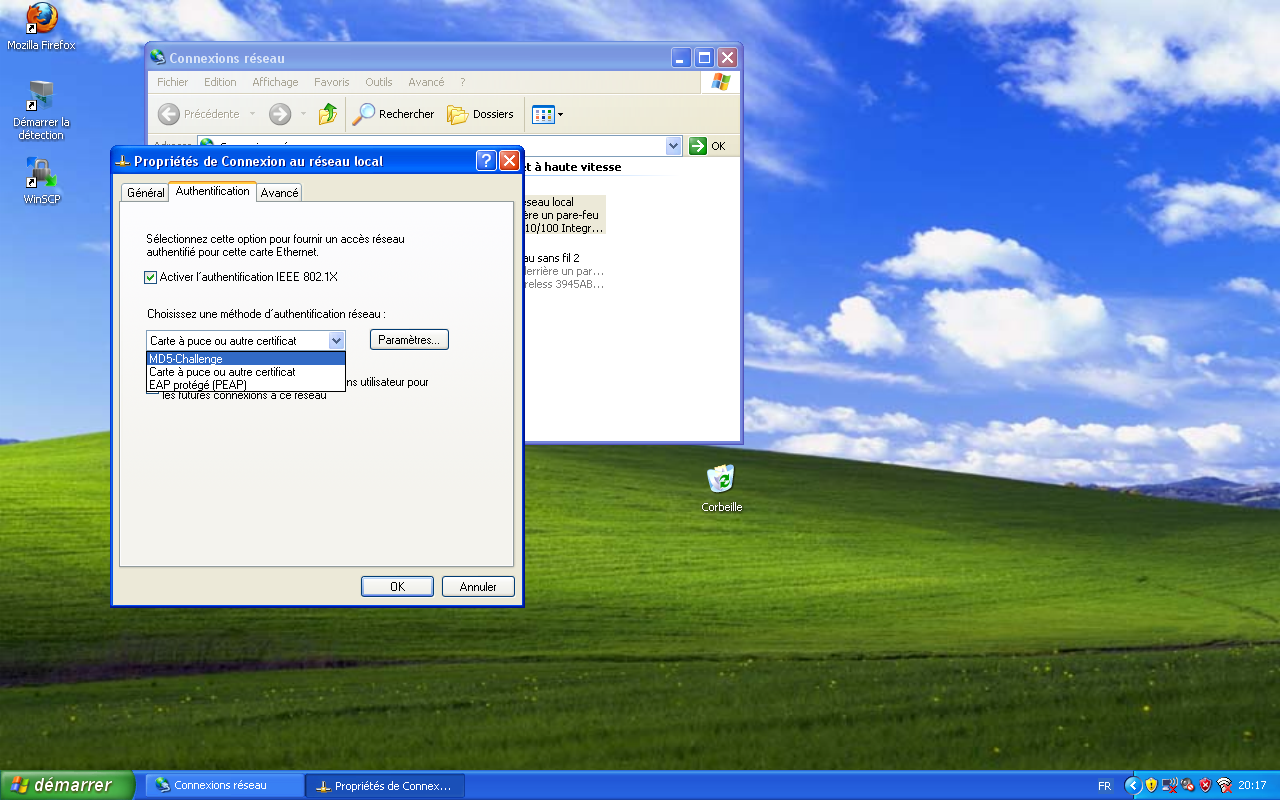
\includegraphics[width=\screenShotSize{}]{imgUser/md5-challenge.PNG}\\
Puis connectez-vous physiquement au reseau.\\
Une info-bulle windows doit apparaître, vous signifiant que l'accès au réseaux requiert des informations supplémentaires.\\
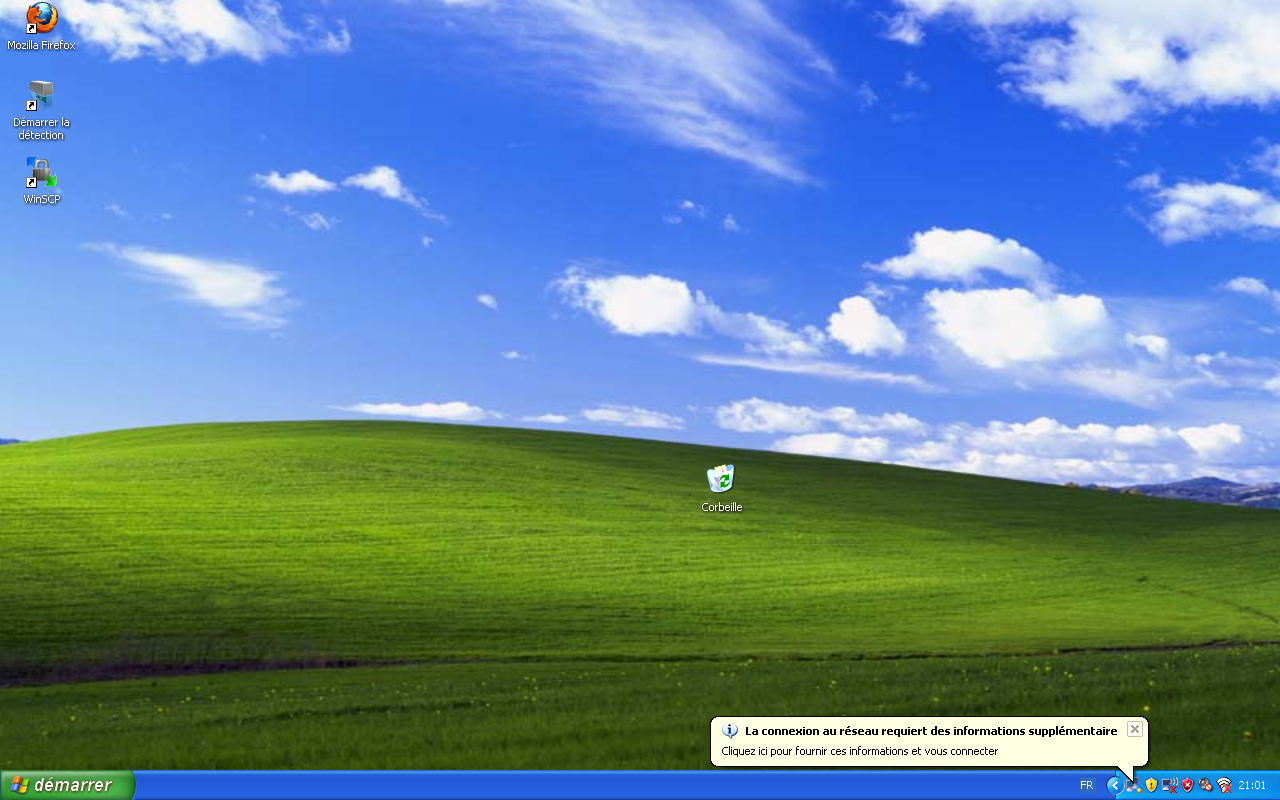
\includegraphics[width=\screenShotSize{}]{imgUser/md5Info.PNG}\\
Après avoir cliqué sur l'info-bulle, il suffit de renseigner ses identifiants.\\
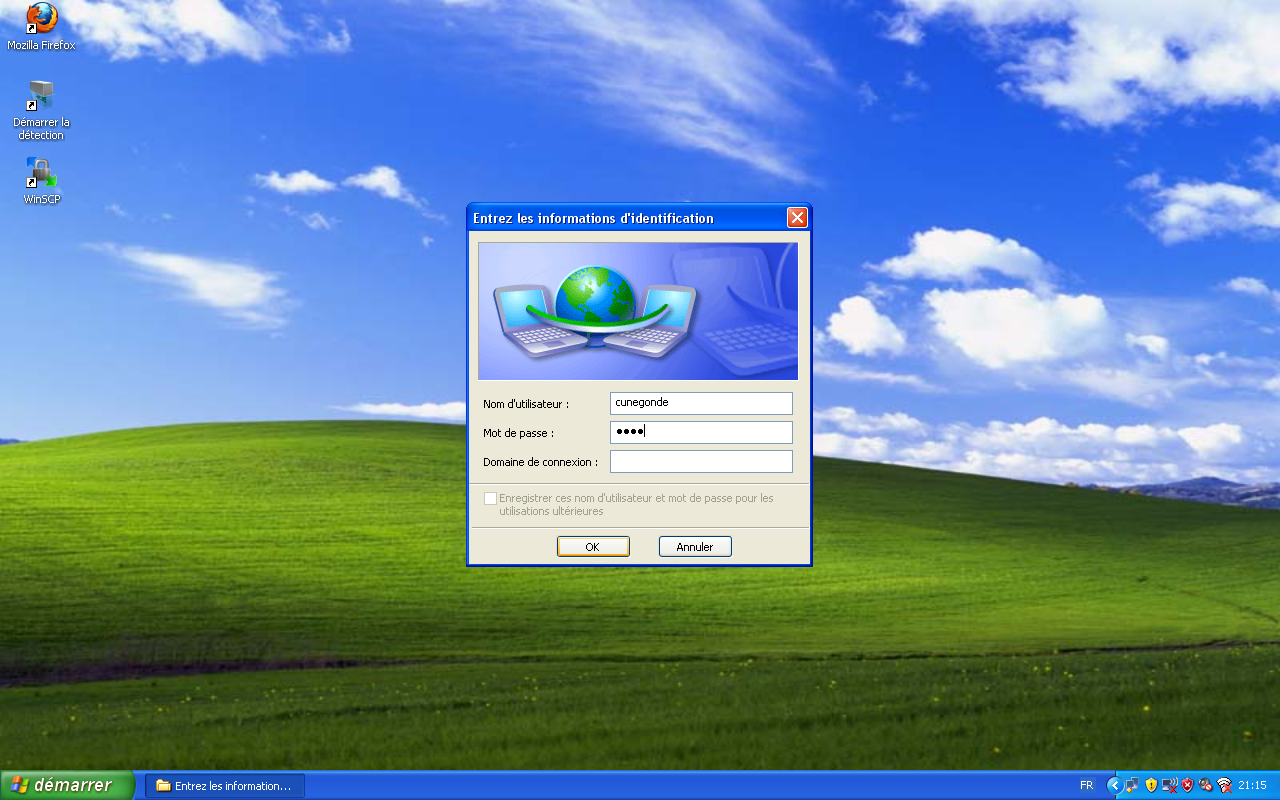
\includegraphics[width=\screenShotSize{}]{imgUser/credentials.PNG}\\
Après avoir validé, la connexion est établie.



\subsection{PEAP}

\subsubsection{Installation du certificat racine}
Pour installer le certificat racine, ouvrer Démarrer puis cliquez sur 'Exécuter' et lancez 'certmgr.msc'.\\
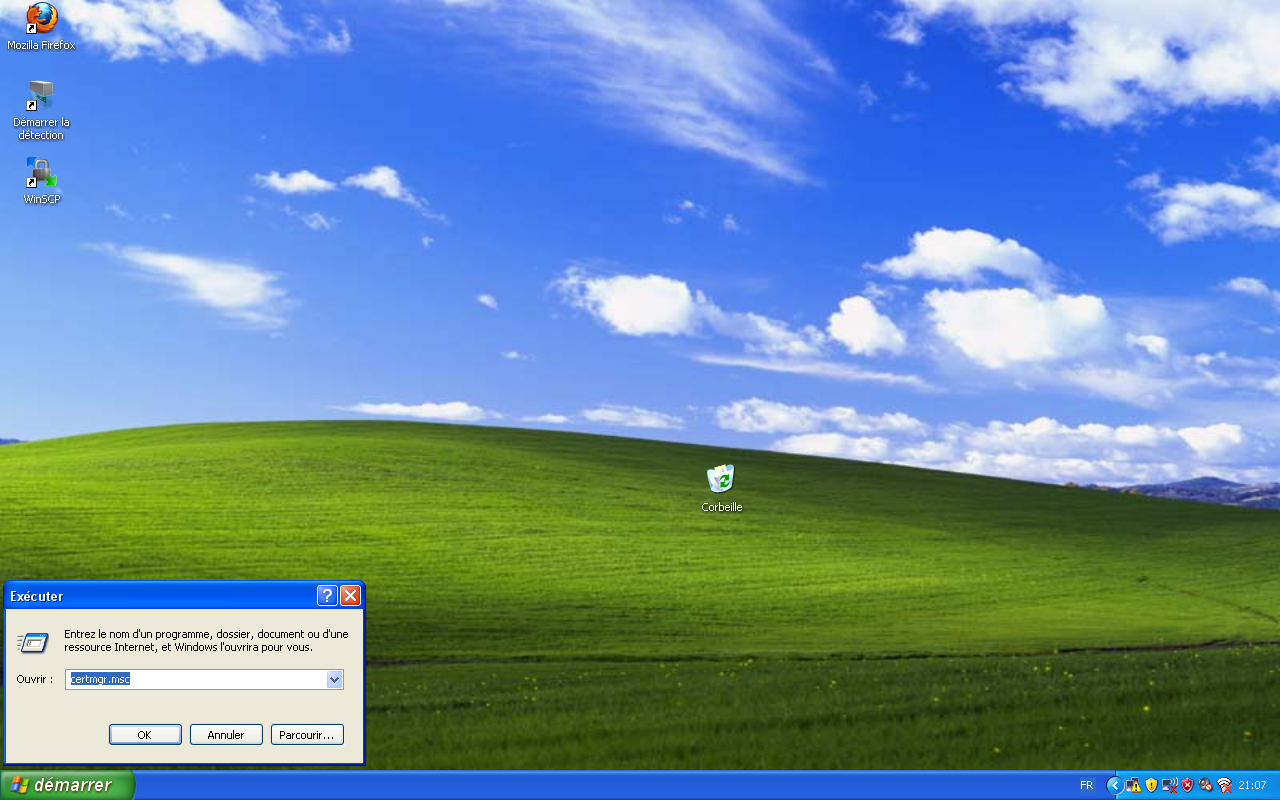
\includegraphics[width=\screenShotSize{}]{imgUser/certmgr.PNG}\\
Double-cliquez ensuite sur les 'Authorités de certification racines de confiance' et faite un clic droit sur le sous-dossier 'Certificats', puis lancez 'toutes les tâches', 'Importer...'.\\
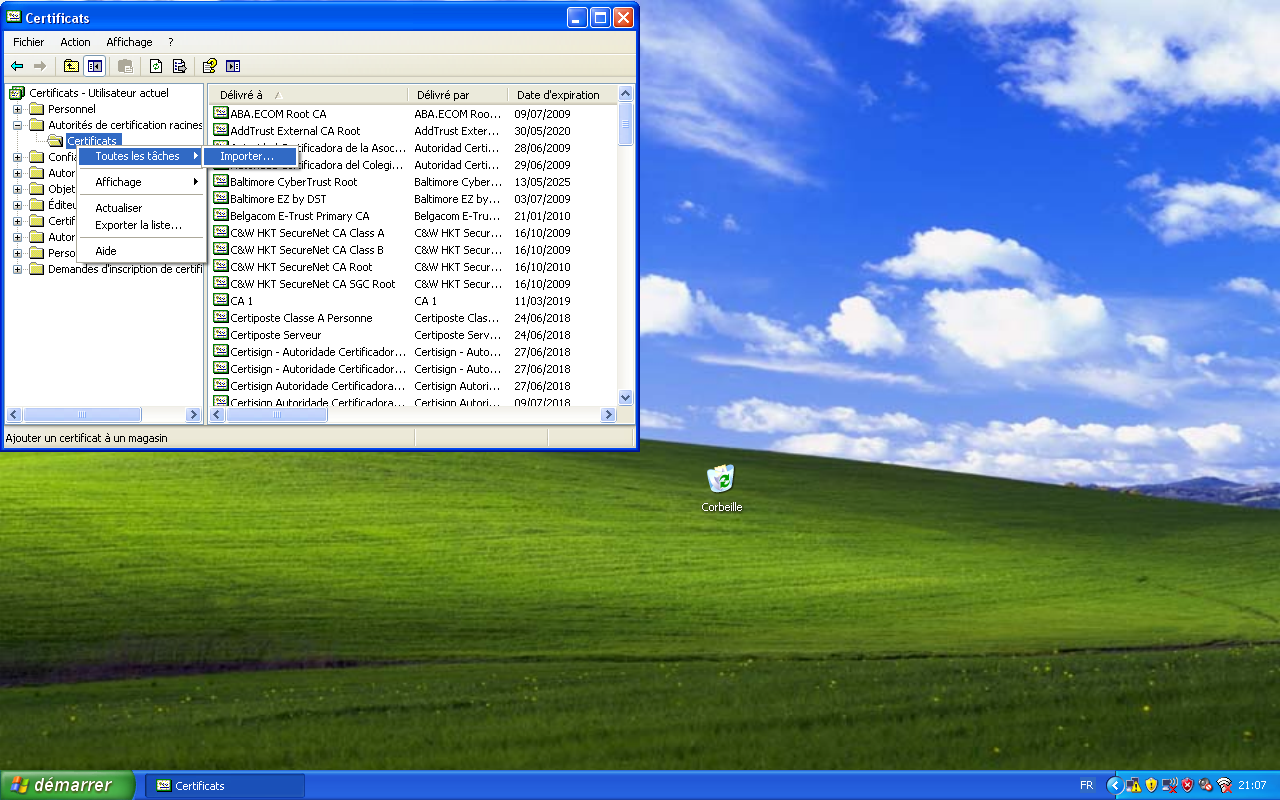
\includegraphics[width=\screenShotSize{}]{imgUser/importCacert.PNG}\\
Cliquez suivant sur le premier panneau proposé. Puis sélectonnez votre fichier grâce au bouton 'Parcourir...'.\\
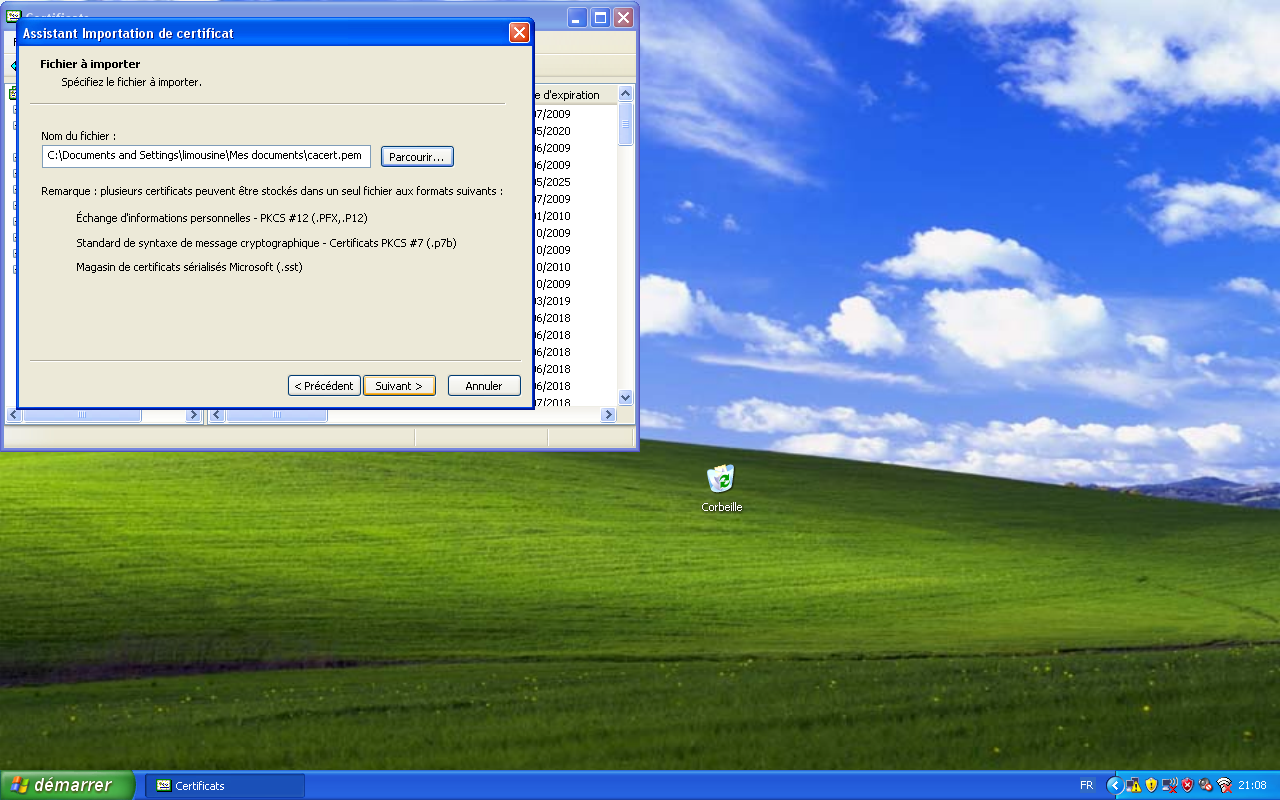
\includegraphics[width=\screenShotSize{}]{imgUser/importCacertFile.PNG}\\
Cliquez sur suivant. Le panneau suivant vous demande de configurer le magasin dans lequel le certificat sera importé. Ici, le bon magasin est déjà choisi (Authorité de certification racines de confiance). Cliquez donc sur OK.\\
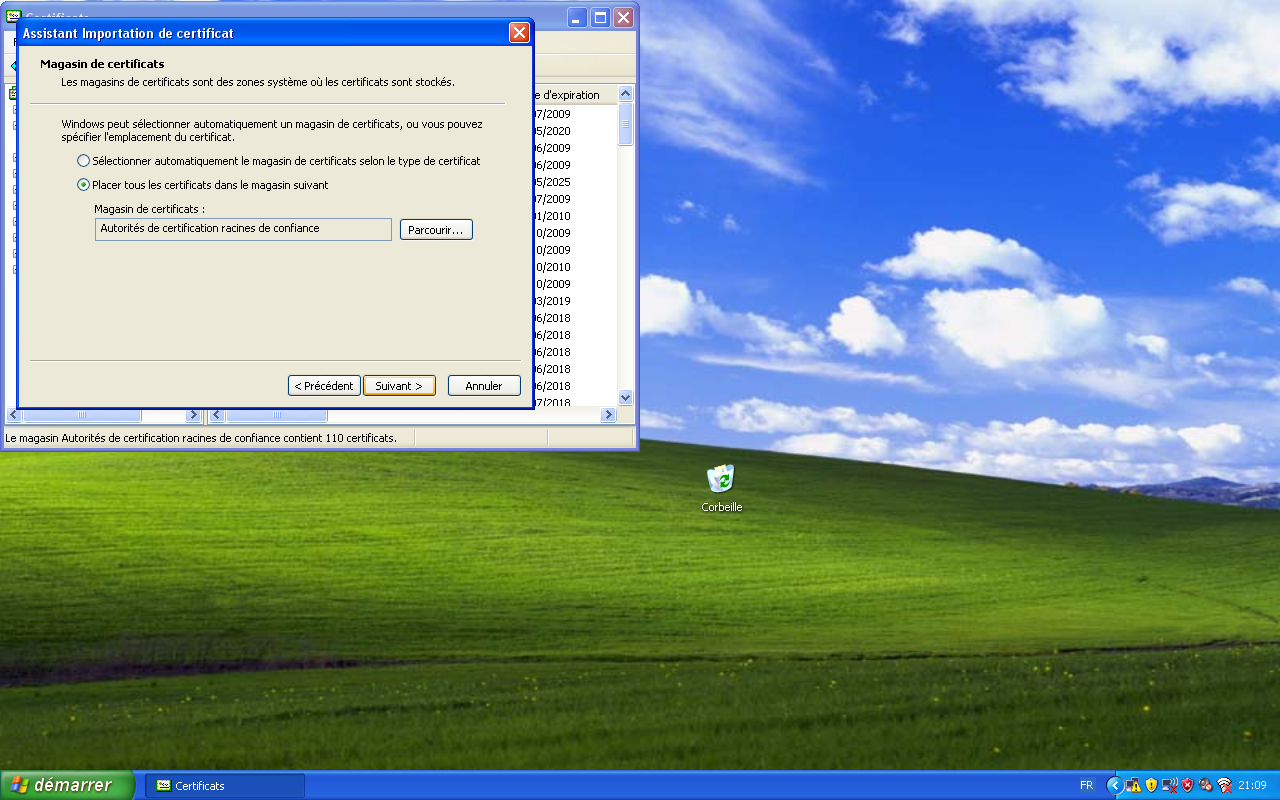
\includegraphics[width=\screenShotSize{}]{imgUser/importCacertStorage.PNG}\\
Cliquez sur suivant. Le dernier panneau permet de terminer l'installation. Cliquez donc sur Terminer.\\
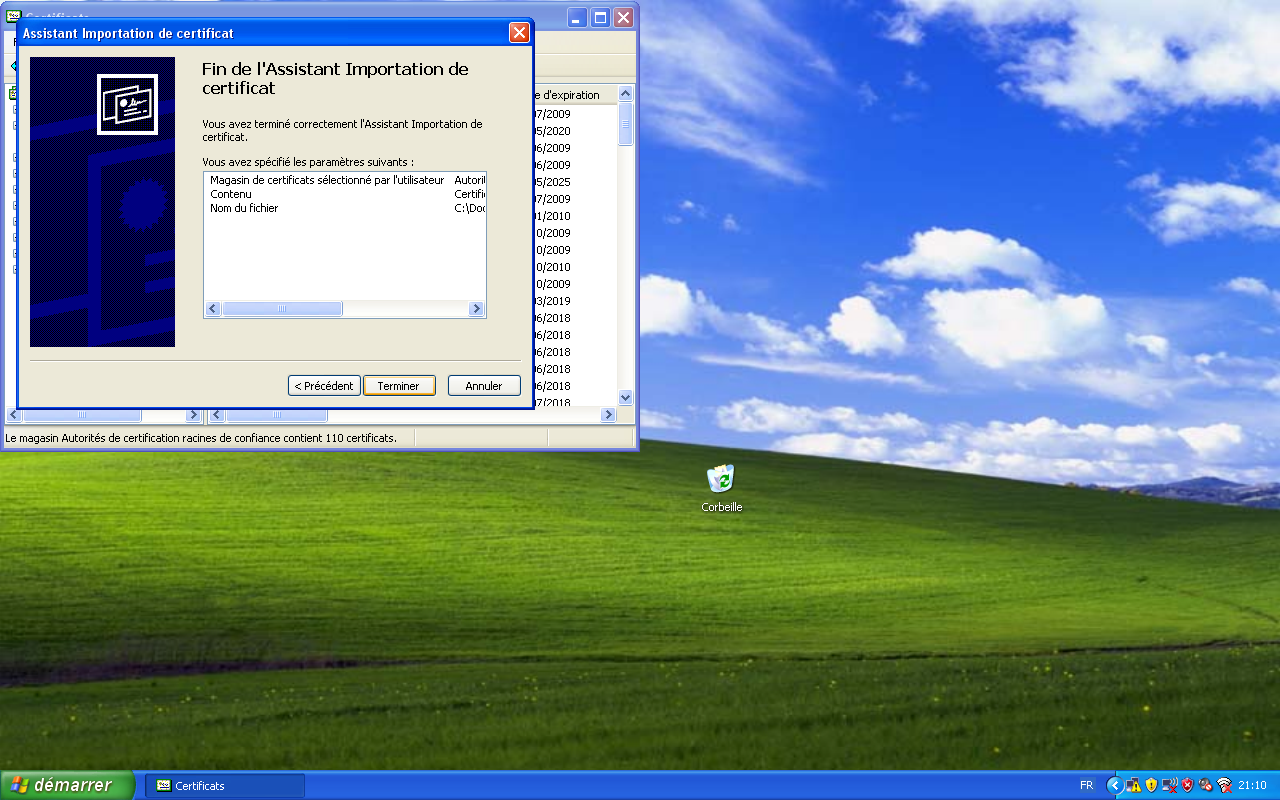
\includegraphics[width=\screenShotSize{}]{imgUser/importCacertFinish.PNG}\\
Un message d'alerte s'ouvre donc pour vous demander confirmation de l'import d'un nouveau certificat racine. Vous pouvez d'ailleurs voir apparaître le nom de l'autorité de certification. (Ici, PoilCorp).\\
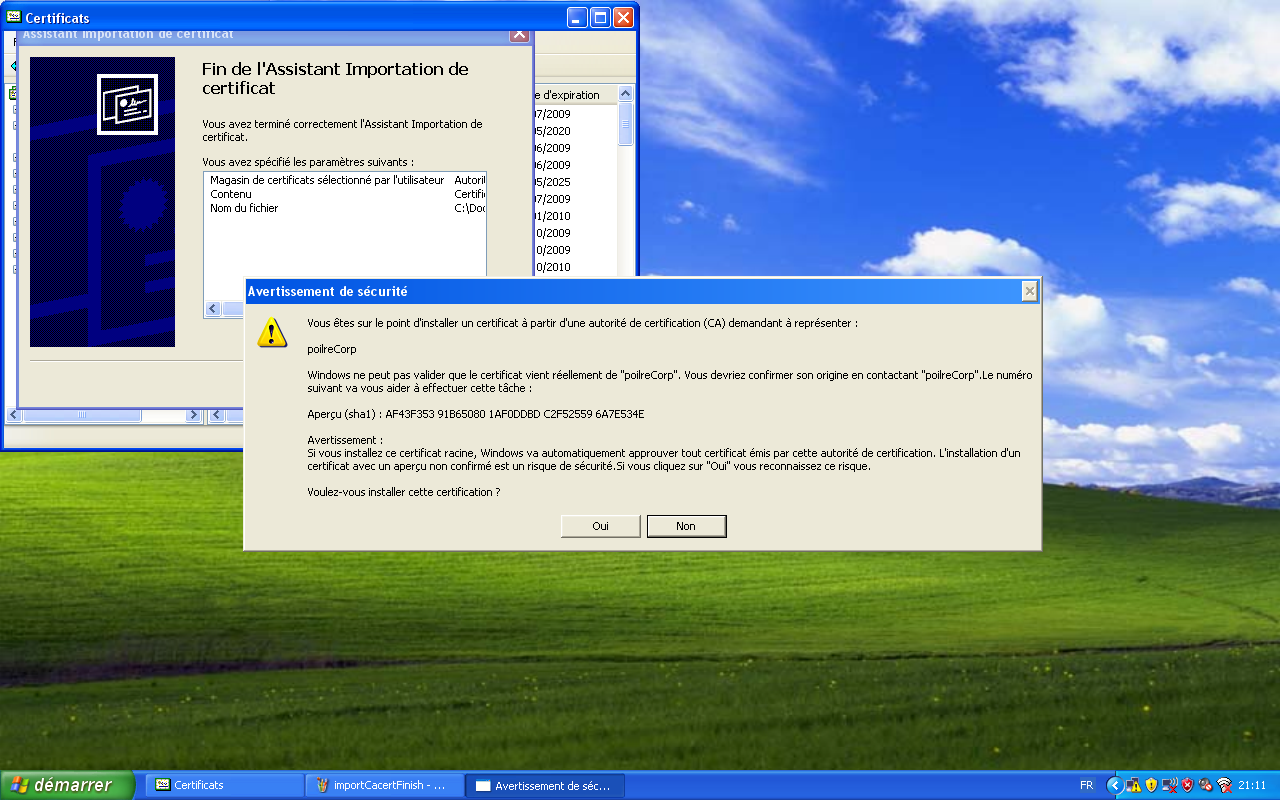
\includegraphics[width=\screenShotSize{}]{imgUser/importCacertAuthorize.PNG}\\
Authorisez cet import ('oui').
Puis validez et quittez toutes les fenêtres ouvertes.

\subsubsection{Paramétrage du PEAP}
Allez dans le panneau des connections.\\
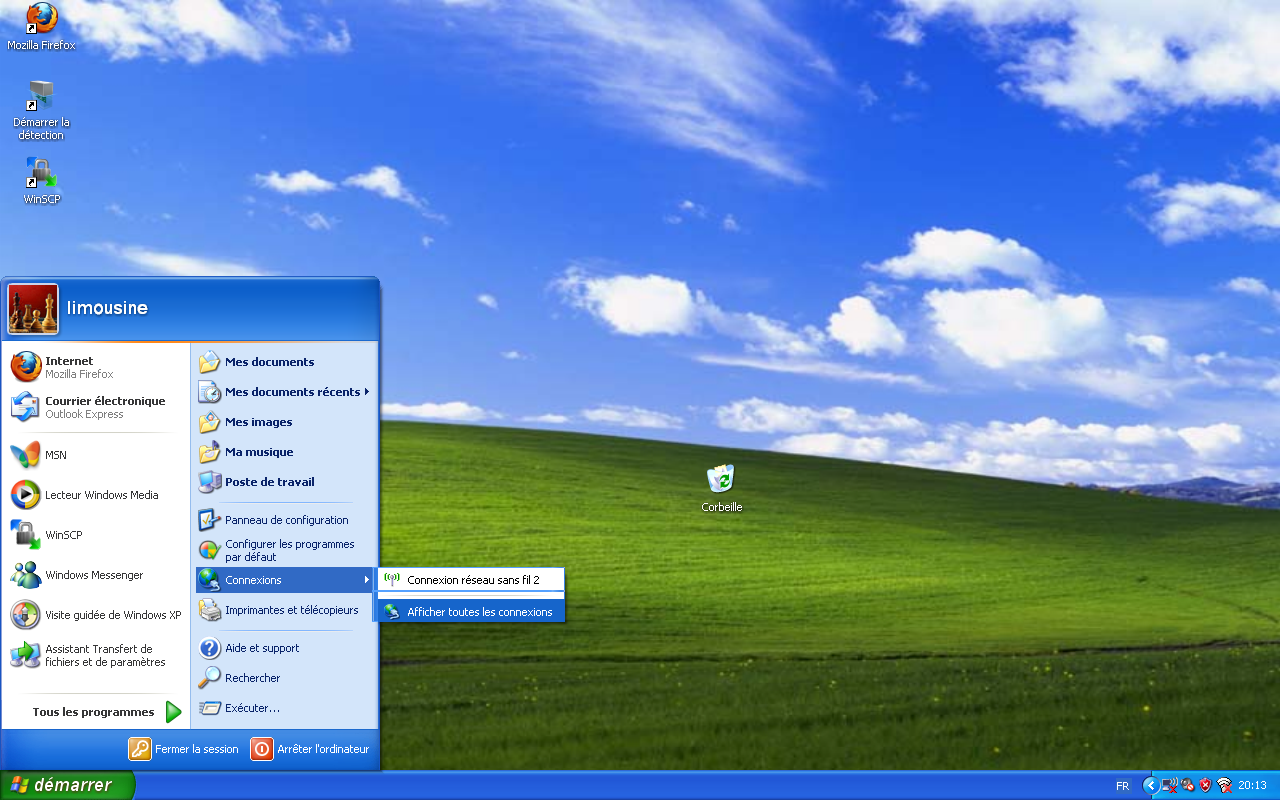
\includegraphics[width=\screenShotSize{}]{imgUser/connections.PNG}\\
Puis effectuez un clic droit sur la connexion que vous utilisez pour accéder au reseaux, et ouvrez les propriétés de la connexion.\\
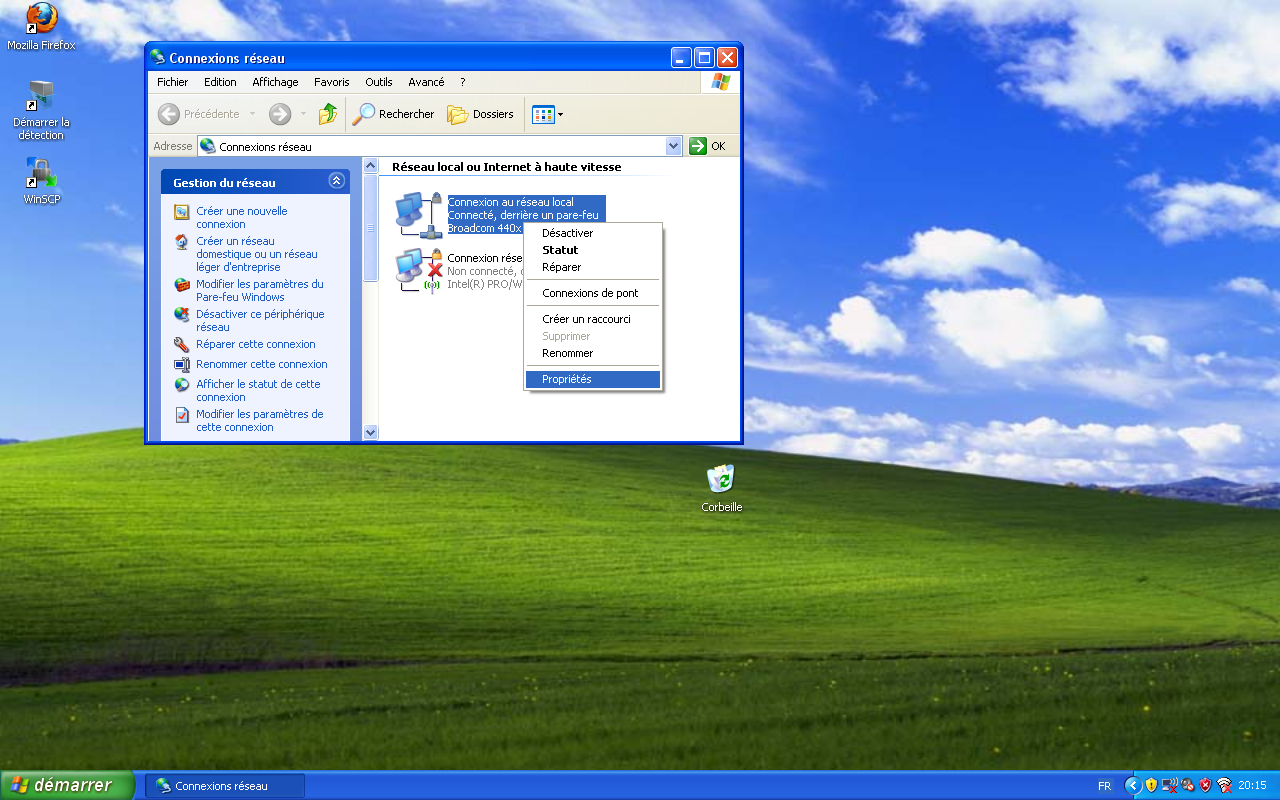
\includegraphics[width=\screenShotSize{}]{imgUser/connectionProperties.PNG}\\
Choisissez alors 'EAP protégé (PEAP)' dans l'onglet 'Authentification'.\\
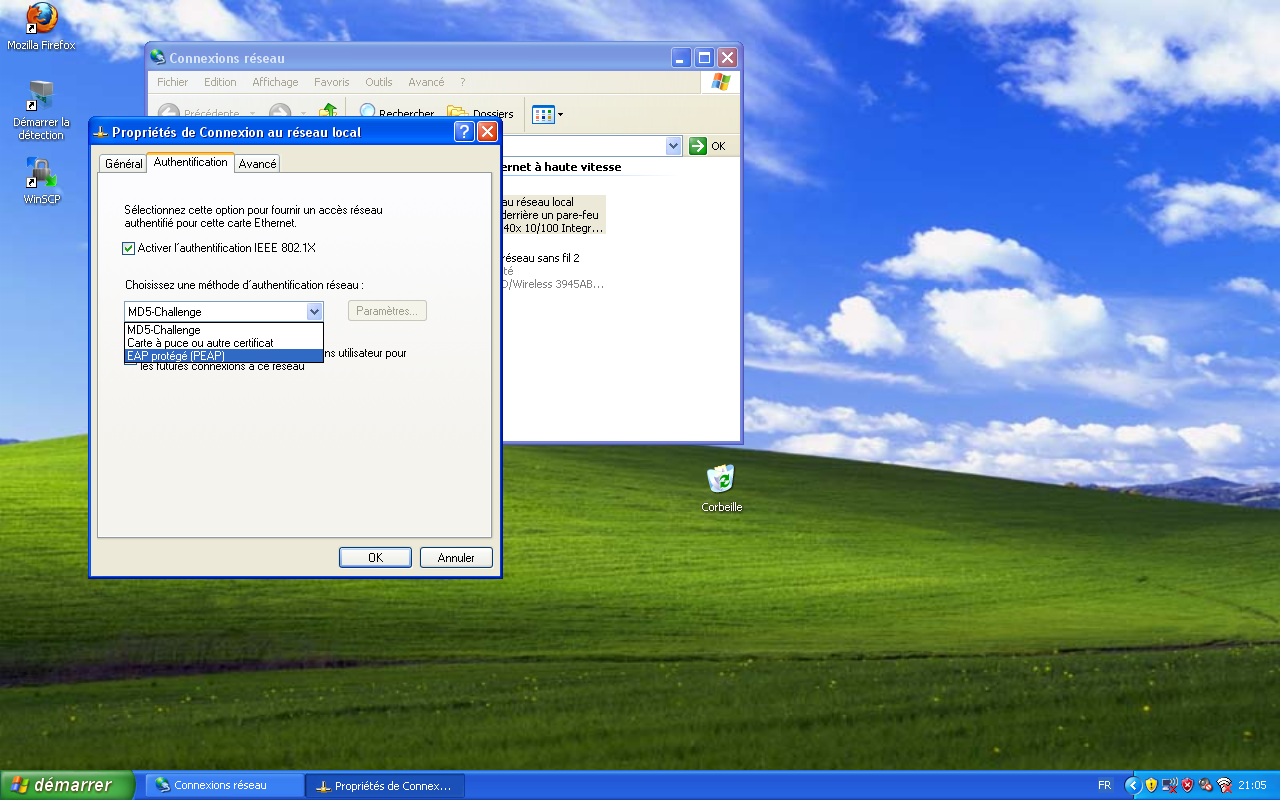
\includegraphics[width=\screenShotSize{}]{imgUser/peap.PNG}\\
Cliquez ensuite sur le bouton 'Paramètres...' à coté de l'option PEAP et cochez votre authorité de certification dans la liste présentée.\\
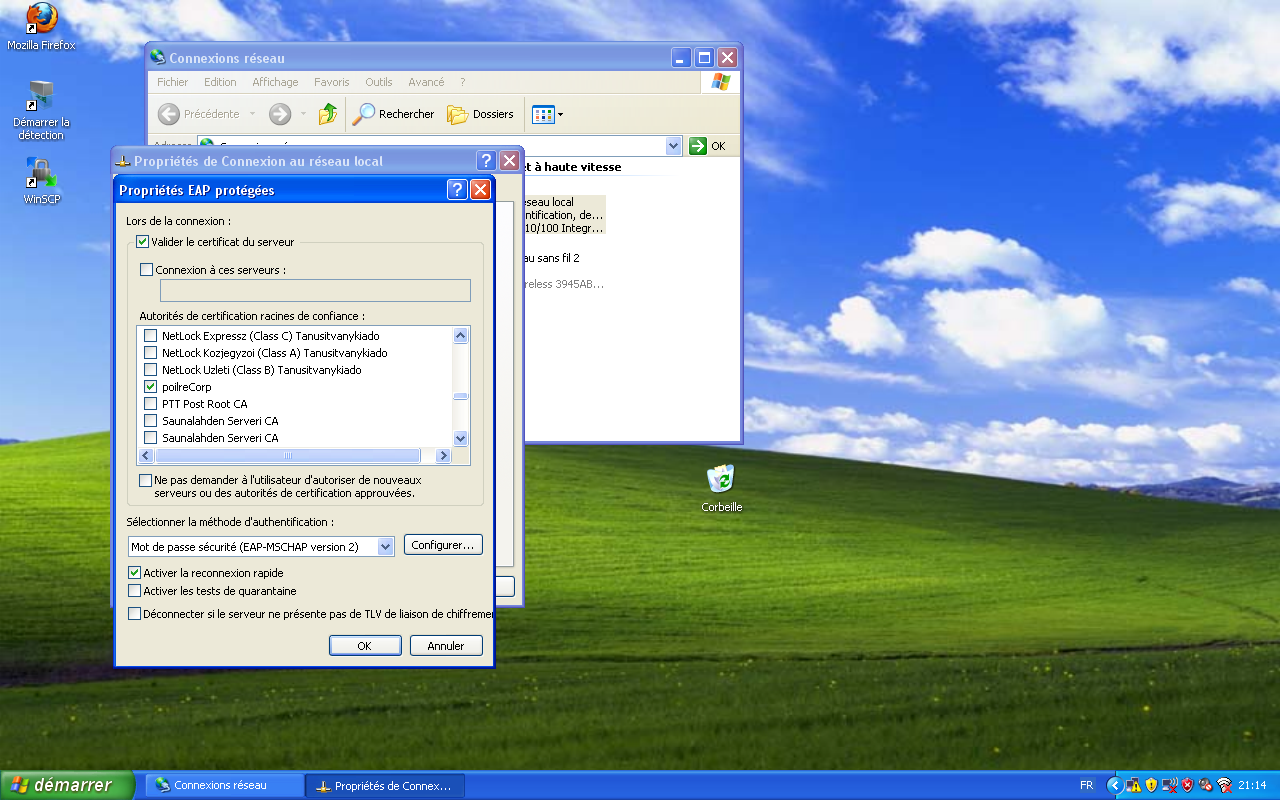
\includegraphics[width=\screenShotSize{}]{imgUser/peapParams.PNG}\\
Cliquez ensuite sur le bouton 'Configurer...' à coté du champs présentant la méthode d'authentification (Mot de passe sécurité (EAP MSCHAP Version 2)).\\
Décochez alors l'utilisation du nom de session, à moins que celui-ci soit effectivement celui utilisé par votre administrateur lors de la création du certificat.\\
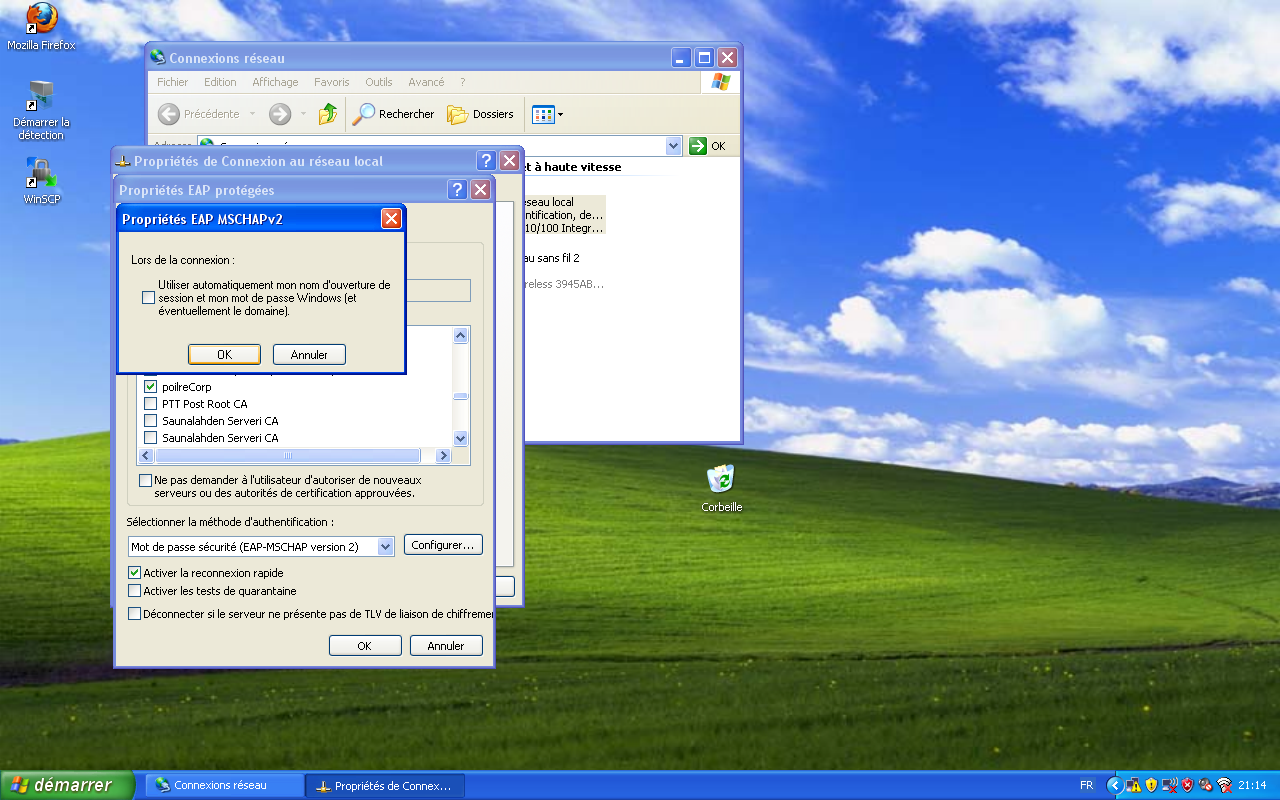
\includegraphics[width=\screenShotSize{}]{imgUser/peapParamsConfig.PNG}\\
Puis validez et fermez toutes les fenêtres ouvertes.
Connectez-vous physiquement au reseau.\\
Une info-bulle windows doit apparaître, vous signifiant que l'accès au réseaux requiert des informations supplémentaires.\\
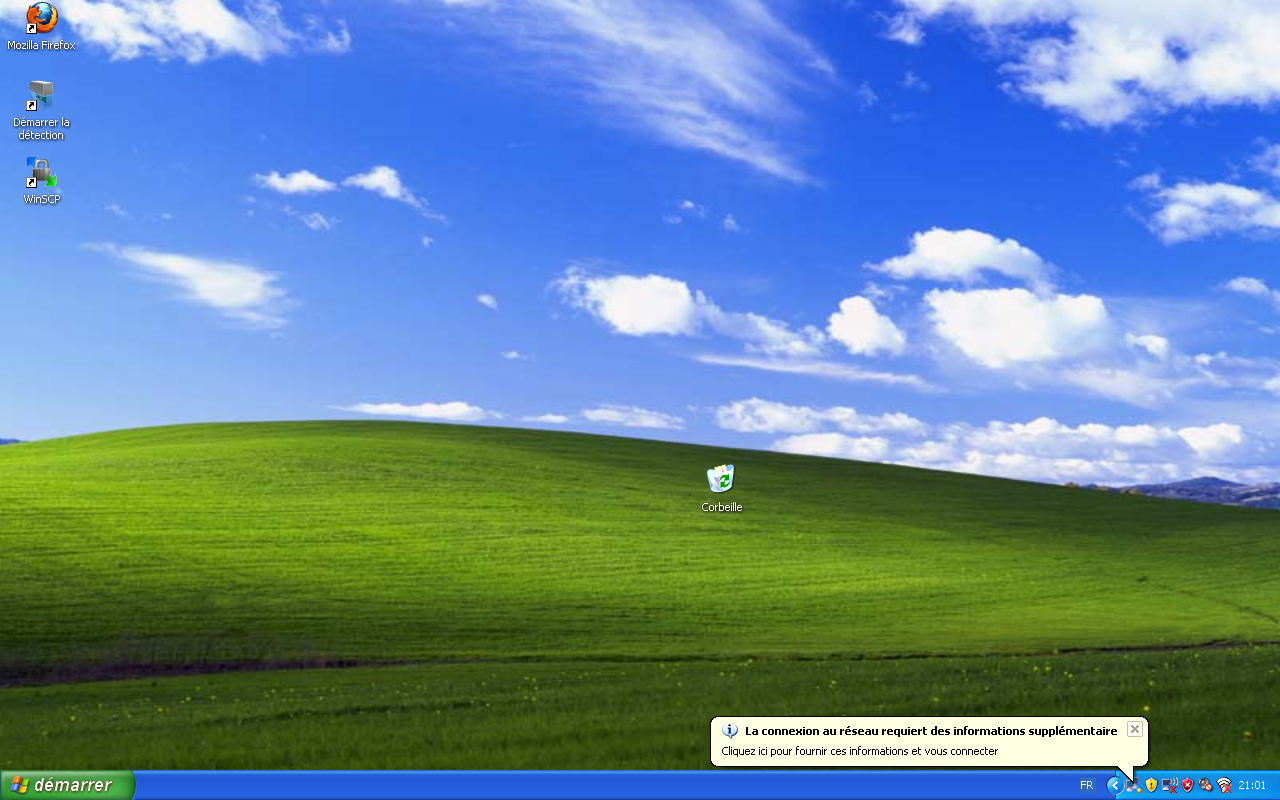
\includegraphics[width=\screenShotSize{}]{imgUser/md5Info.PNG}\\
Après avoir cliqué sur l'info-bulle, il suffit de renseigner ses identifiants.\\
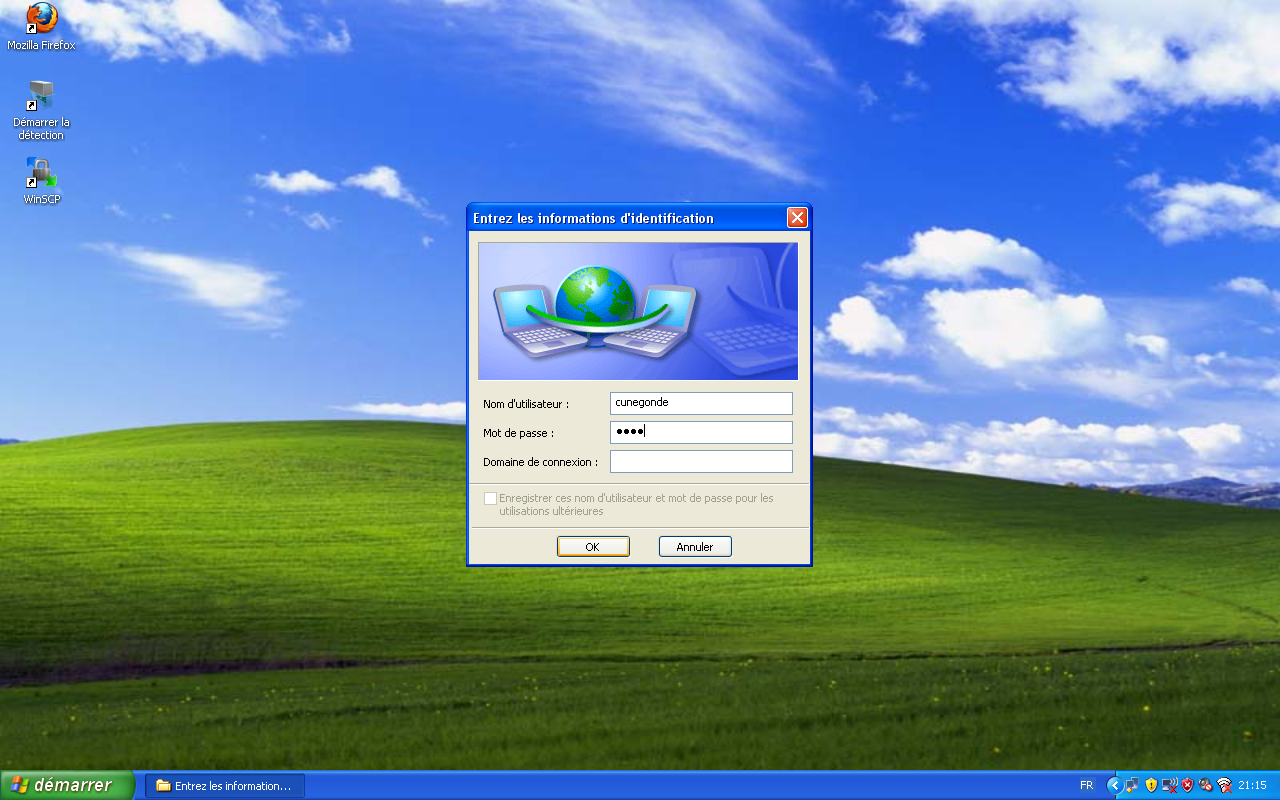
\includegraphics[width=\screenShotSize{}]{imgUser/credentials.PNG}\\
Après avoir validé, la connexion est établie.



\subsection{TLS}

Si ce n'est pas fait, commencez par installer le certificat racine (ci-dessus, section PEAP).

\subsubsection{Installation du certificat Client}
Pour installer le certificat client au format p12, il vous suffit de double-cliquer dessus. Le même assistant que celui utilisé pour l'installation du certificat racine apparait.\\
Cliquez sur suivant lors du premier panneau. Cliquez sur suivant sur le panneau suivant (Le chemin du fichier est déjà bon).\\
Sur le panneau suivant, un mot de passe vous est demandé. Laissez le champs vide et cliquez sur suivant.\\
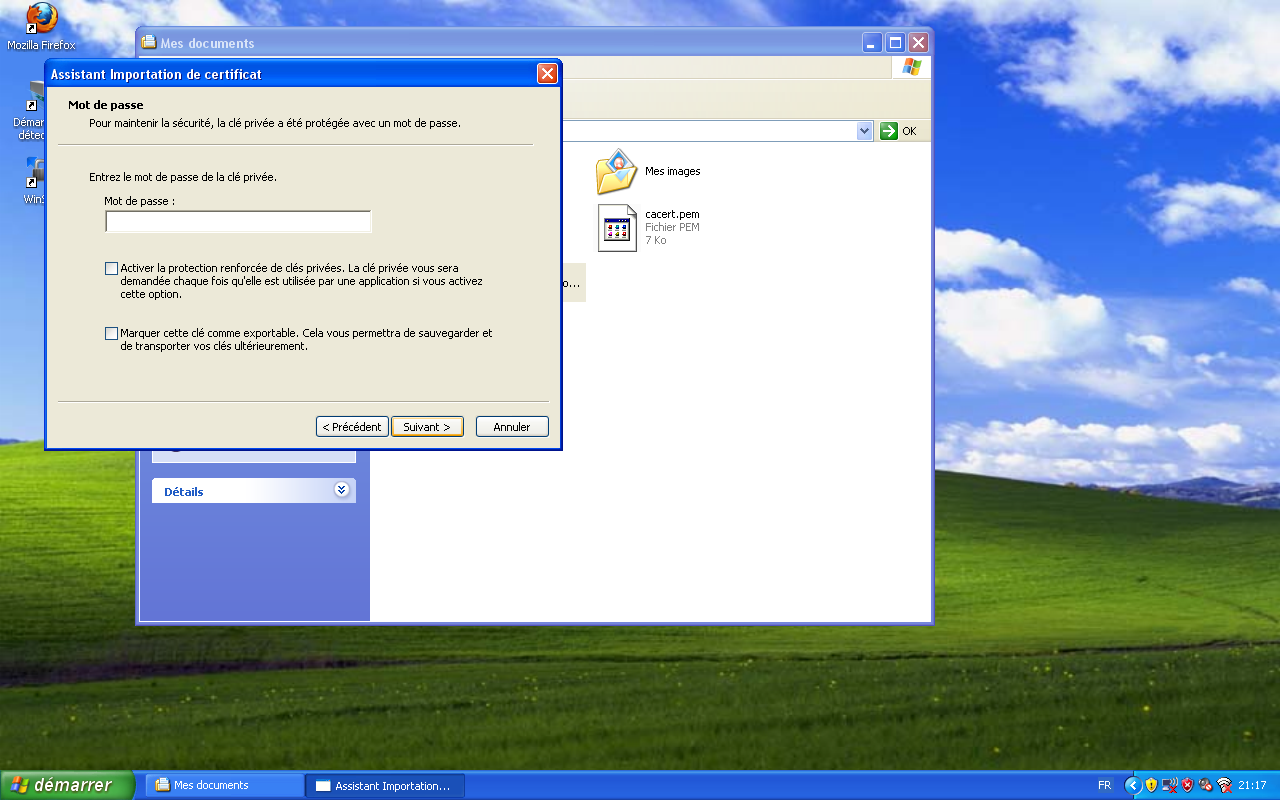
\includegraphics[width=\screenShotSize{}]{imgUser/importClient.PNG}\\
Cliquez ensuite sur suivant une nouvelle fois. La selection automatique du magasin est en effet adaptée pour ce cas. \\
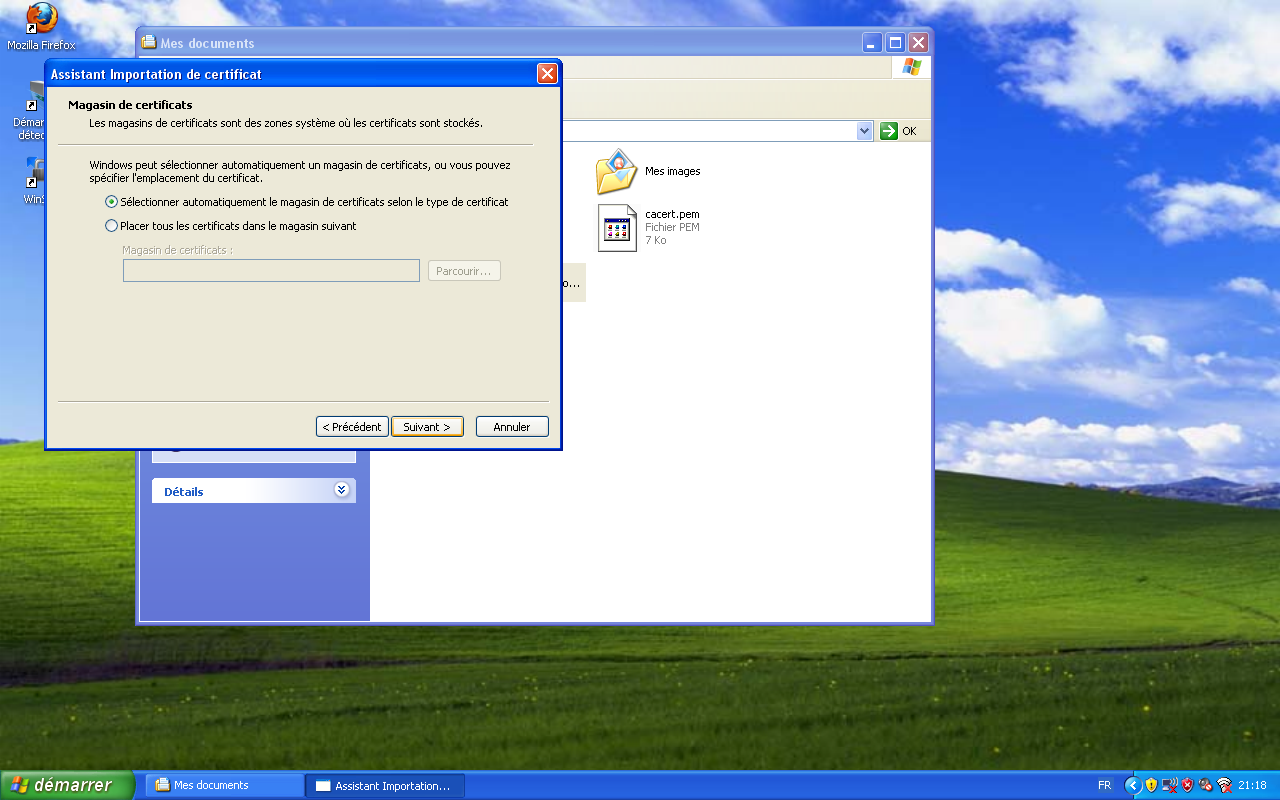
\includegraphics[width=\screenShotSize{}]{imgUser/importClient2.PNG}\\
Cliquez enfin sur Terminer.\\

\subsubsection{Paramétrage du TLS}
Allez dans le panneau des connections.\\
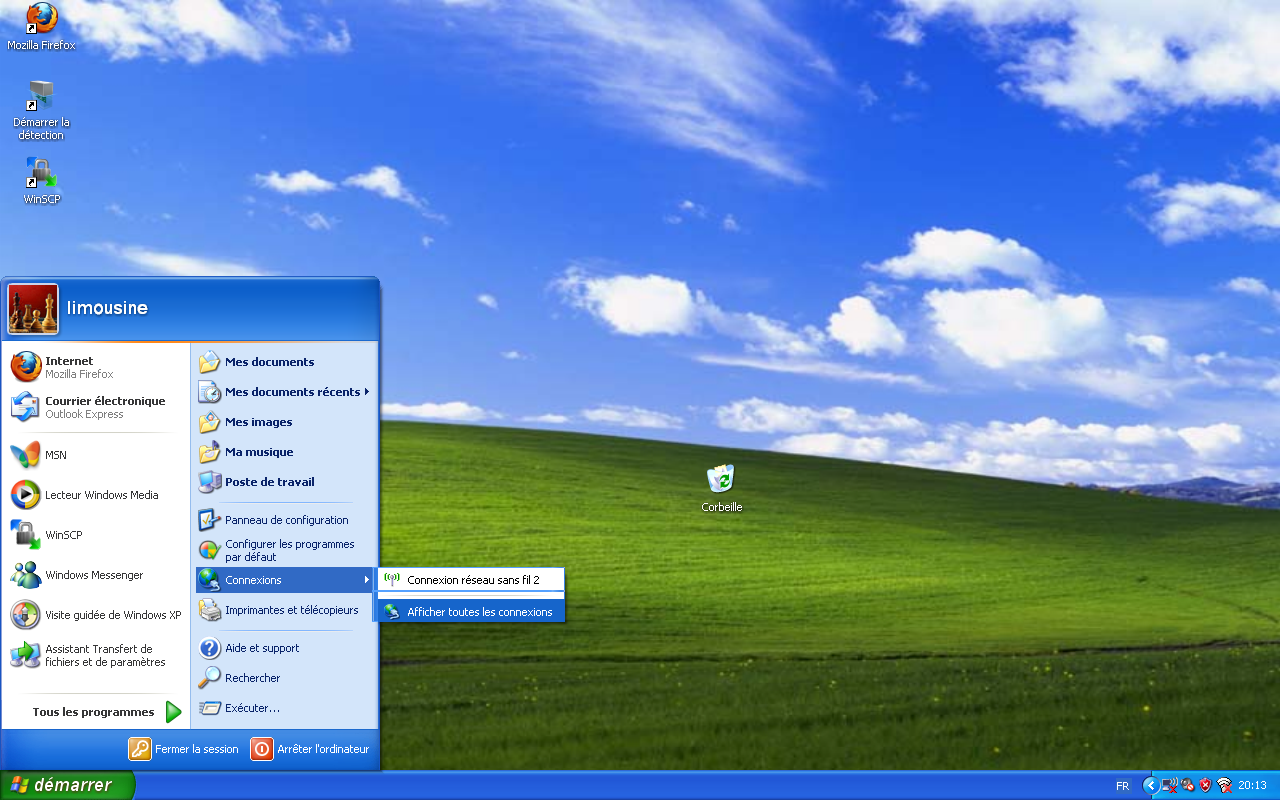
\includegraphics[width=\screenShotSize{}]{imgUser/connections.PNG}\\
Puis effectuez un clic droit sur la connexion que vous utilisez pour accéder au reseaux, et ouvrez les propriétés de la connexion.\\
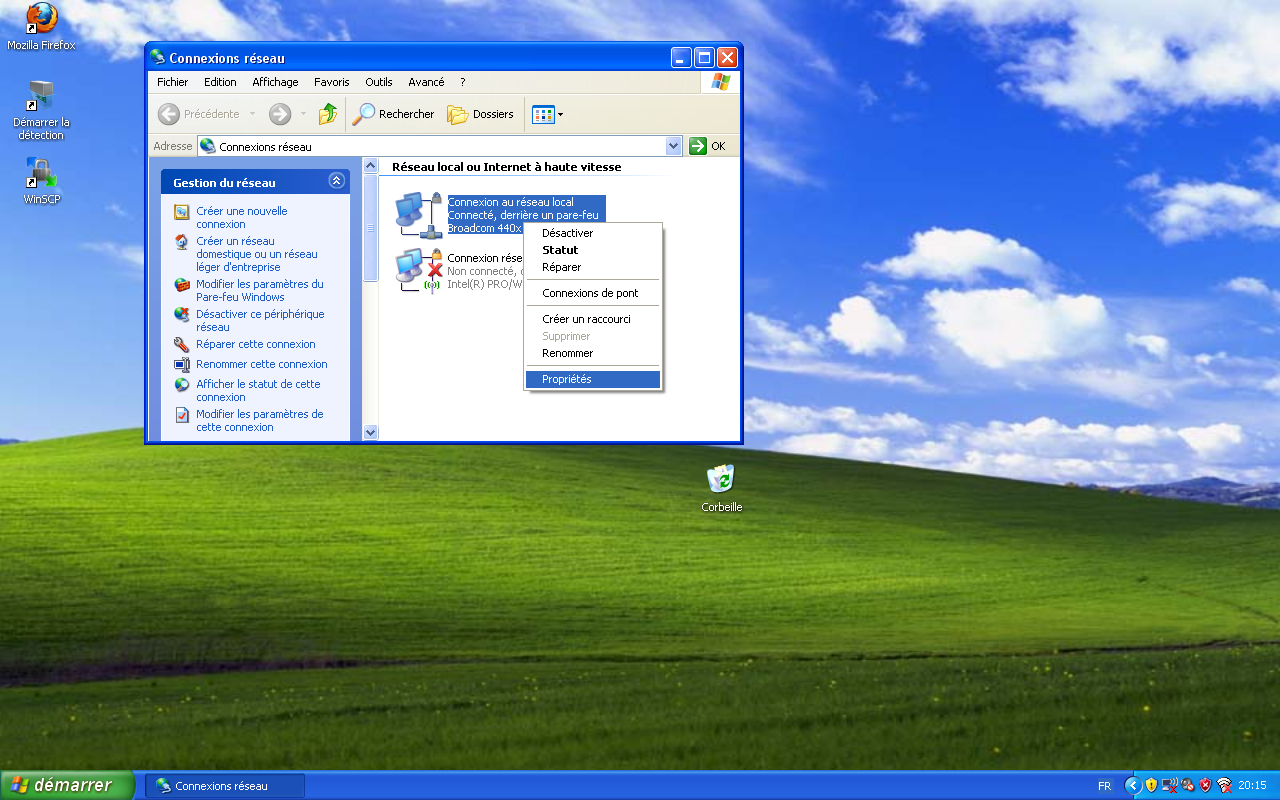
\includegraphics[width=\screenShotSize{}]{imgUser/connectionProperties.PNG}\\
Choisissez alors 'Carte à puce ou autre certificat' dans l'onglet 'Authentification'.\\
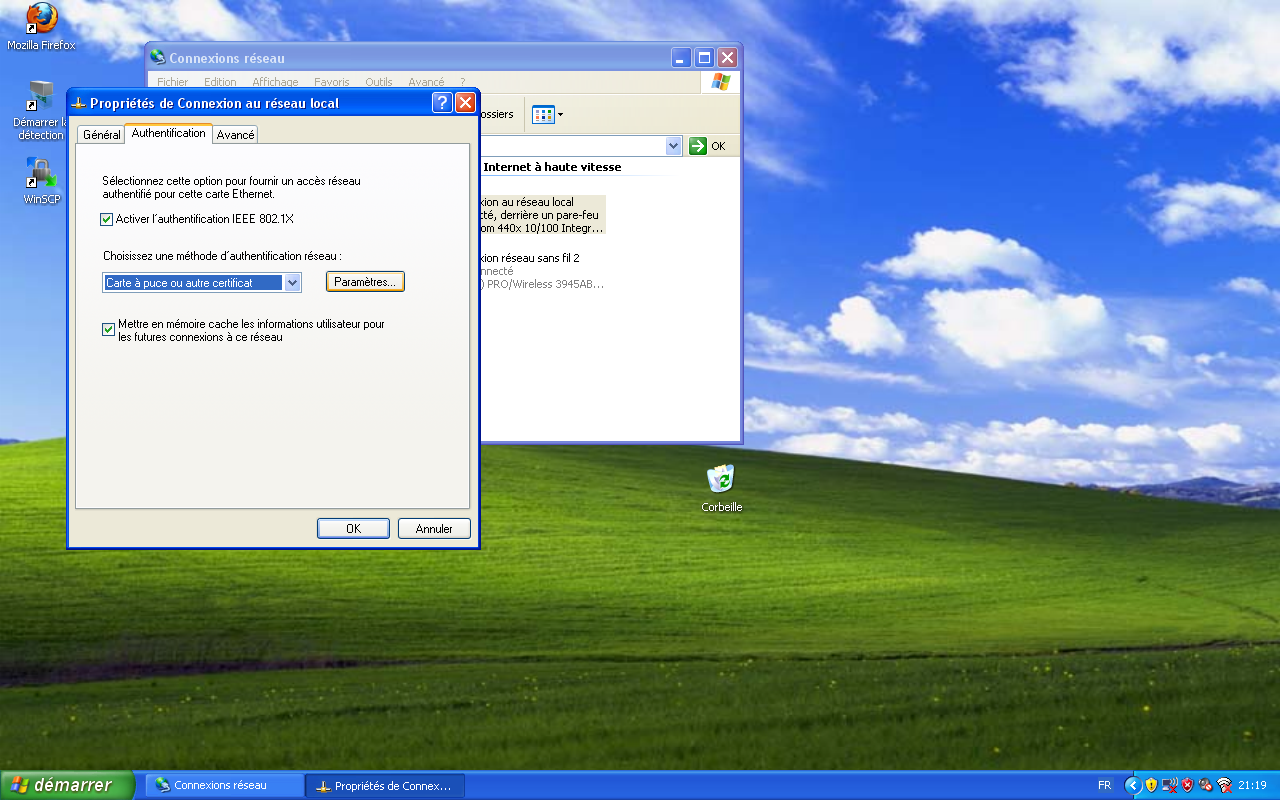
\includegraphics[width=\screenShotSize{}]{imgUser/tls.PNG}\\
Cliquez ensuite sur le bouton 'Paramètres...' à coté de l'option PEAP et cochez votre authorité de certification dans la liste présentée.\\
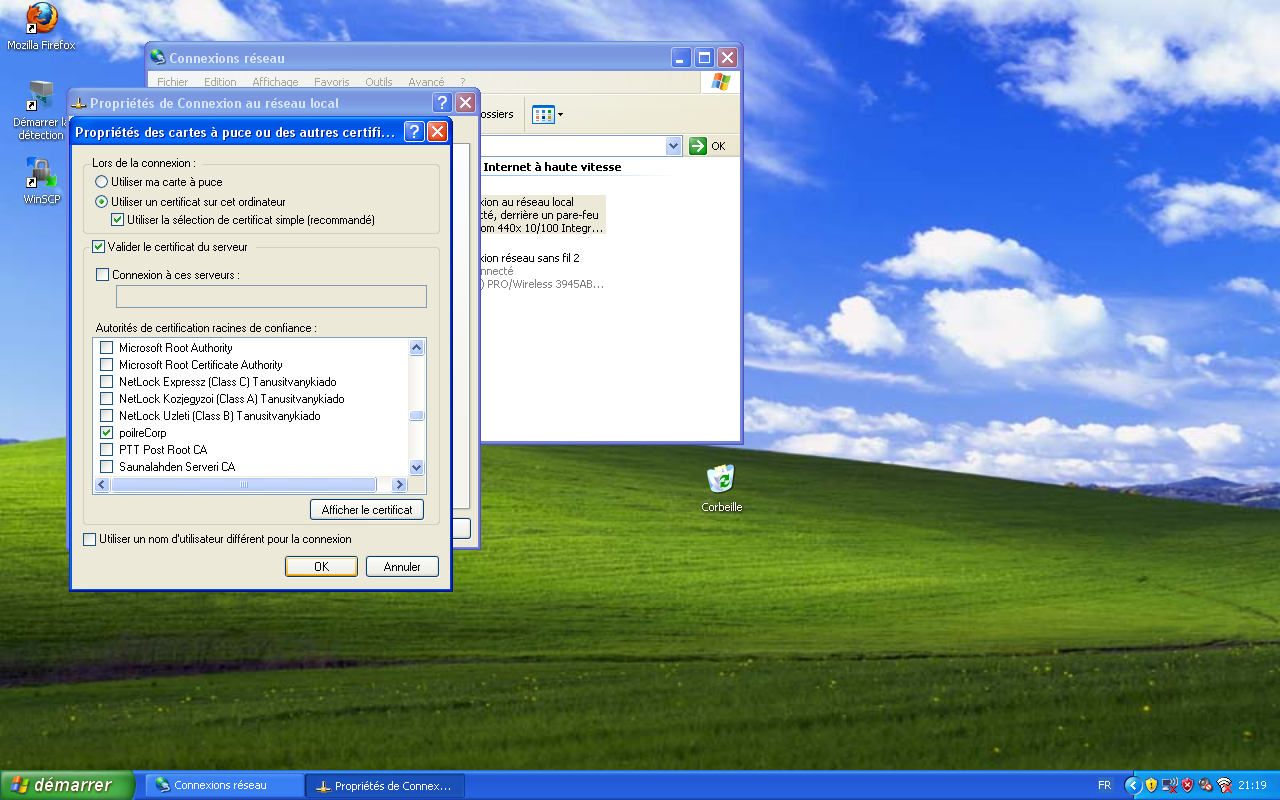
\includegraphics[width=\screenShotSize{}]{imgUser/tlsParams.PNG}\\
Validez et quitez enfin toutes les fenêtres ouvertes.\\
Connectez-vous physiquement au réseau. La connection est établie.






